\providecommand{\pdfxopts}{a-1b,cyrxmp}
\providecommand{\thisyear}{2022}
\immediate\write18{rm \jobname.xmpdata}%  uncomment for Unix-based systems
\begin{filecontents*}{\jobname.xmpdata}
	\Title{Лабораторные работы «Цифровая электроника» с использованием «MexBIOS Development Studio 6.21»\textemdash\thisyear}
\Author{Артем Николаевич Прокшин}
\Creator{pdfTeX + pdfx.sty with options \pdfxopts }
\Subject{Лабораторные работы по дисциплине «Цифровая электроника» с использованием российского программного обеспечения
	«MexBIOS Development Studio 6.21»}
\Keywords{ковариантныые и контравариантрные координаты, MexBIOS Development Studio, электричесие машины}
\CoverDisplayDate{март \thisyear}
\CoverDate{2022-09-08}
\Copyrighted{True}
\Copyright{Public Domain}
\CopyrightURL{http://github.com/trot-t}
\Creator{pdfTeX + pdfx.sty with options \pdfxopts }
\end{filecontents*}

\documentclass[14pt]{beamer}

\pdfcompresslevel=9

\usepackage[\pdfxopts]{pdfx}[2016/03/09]
\PassOptionsToPackage{obeyspaces}{url}
\let\tldocrussian=1  % for live4ht.cfg

\usepackage[T2A]{fontenc}
\usepackage[utf8]{inputenc}
\usepackage[english,russian]{babel}
\usepackage{booktabs}
\usepackage{tikz}
\usepackage[european,cuteinductors,smartlabels]{circuitikz}
\usetikzlibrary{arrows.meta, shadows}

\usepackage{amssymb,amsfonts,amsmath,mathtext}
\usepackage{amssymb}
\usepackage{cite,enumerate,float,indentfirst}
\usepackage{cancel}
\usepackage{csquotes}
\newcommand{\quotes}[1]{``#1''}
\usetikzlibrary{calc}

\usepackage{advdate}

%\usepackage{pgfplots}
%\usepackage[left=1cm,right=1cm, top=1cm,bottom=1cm,bindingoffset=0cm]{geometry}

% Beamer — верстаем презентации  https://habrahabr.ru/post/145523/ 
\graphicspath{{images/}}

\usetheme{Pittsburgh}
\usecolortheme{whale}

\setbeamercolor{footline}{fg=blue}
\setbeamertemplate{footline}{
\leavevmode%
\hbox{%
\begin{beamercolorbox}[wd=.333333\paperwidth,ht=2.25ex,dp=1ex,center]{}%
Прокшин А.Н.
\end{beamercolorbox}%
\begin{beamercolorbox}[wd=.333333\paperwidth,ht=2.25ex,dp=1ex,center]{}%
Санкт-Петербург, 2022
\end{beamercolorbox}%
\begin{beamercolorbox}[wd=.333333\paperwidth,ht=2.25ex,dp=1ex,right]{}%
Стр. \insertframenumber{} из \inserttotalframenumber \hspace*{2ex}
\end{beamercolorbox}}%
\vskip0pt%
}

\newcommand{\itemi}{\item[\checkmark]}

	\usefonttheme[onlymath]{serif} % в формулах использовать текст с засечками
\begin{document}
\title{\small{ Лабораторные работы по дисциплине \enquote{Цифровая электроника} с использованием российского программного обеспечения
\enquote{MexBIOS Development Studio 6.21}}}
\author{\small{%
\emph{}~Прокшин Артем Николаевич}}



\institute{Санкт-Петербургский государственный электротехнический университет «ЛЭТИ» им. В.И. Ульянова (Ленина)}
\vspace{30pt}%

\vspace{60pt}%

\AdvanceDate[0] % печатаю в субботу а нужна пятница
%\date{\small{Санкт-Петербург, 2022}}

\AtBeginSection{
	\begin{frame}
		\frametitle{Содержание}
		\tableofcontents[currentsection]
	\end{frame}
}

\begin{frame}
\titlepage	
\end{frame}

%\begin{frame}
%        \frametitle{Содержание}
%        \tableofcontents[currentsection] 
%\end{frame}

%% \begin{frame}
%% \frametitle{\small Цели, к которым стремились при реализации курса} 
%% \begin{itemize}
%%	\item упрощение системы управления с использованием ковариантных (измеряемых) и контравариантных (неизмеряемых) координат;
%% %\item использование дипломных проектов студентов; % предыдущих выпусков;
%% \item создание мобильных лабораторных стендов; % по тематике кафедры с перспективой на использование российских разработок;
%% \item использование российского программного обеспечения;
%% \item использование российских микроконтроллеров в части задач 
%% %\item оформление УМКД;
%% %\item ... будет сформулирована в результатах.
%%\end{itemize}
%% \end{frame}

\begin{frame}
\begin{itemize}
\item Упрощение описания системы управления:
 \begin{itemize}
 \item геометрическое описание совпадающее с физическим смыслом
 \end{itemize}
 
 \item Российское программное обеспечение в котором \enquote{не надо знать программирование}

 \item Наличие объекта управления и драйверов:
    \begin{itemize}
    \item электрический мотор
    \item солнечная панель
    \item промышленная сеть
    \item инвертор напряжения
    \end{itemize}

 \item Доступность микроконтроллеров
\end{itemize}
\end{frame}



\frame{
\frametitle{\small длина вектора, ковариантные и контрaвариантные координаты}

\centering
\begin{circuitikz}
        \newcommand{\I}{3.2}
        \newcommand{\teta}{120}
        \newcommand{\alfa}{25}

        \newcommand{\X}{\I*cos(\alfa)}
        \newcommand{\Y}{\I*sin(\alfa)}
        \newcommand{\Xaxe}{4.6}
        \newcommand{\Yaxe}{4}

        % ось
        \draw[very thin,->,>=latex] (0,0) -- ({\Xaxe},0) node[right] {\only<1>{\small $I_A$}};
        \draw[very thin, ->,>=latex] ({1*cos(\teta-180)},{1*sin(\teta-180)}) -- ({\Yaxe*cos(\teta)},{\Yaxe*sin(\teta)}) node[right] {\small $I_B$};

        \draw[->,red,thick,>=latex] (0,0) -- ({\I*cos(\alfa)}, {\I*sin(\alfa)}) node[above right] {$\vec{i}$};
        % проекция на ось Х
        \draw[very thin, dashed] ({\X},{\Y}) -- ({\X-\Y*cos(\teta)/sin(\teta)}, 0) node[below right] {\small $i^A$};

        \draw[thin, dotted] ({\X},{\Y}) -- ({\X},0) node[below] {\small $i_A$};
        % проекция на ось Y

        \draw[very thin, dashed] ({\X}, {\Y}) -- ( {\Y*cos(\teta)/sin(\teta)} ,{\Y}) node[left] {\small $i^B$};
        % перпендикуляр на ось Y
        \newcommand{\perpend}{\I*cos(\teta-\alfa)}
        \draw[thin,dotted] ({\X}, {\Y}) -- ({\perpend*cos(\teta)},{\perpend*sin(\teta)}) node[below left] {\small $i_B$};
\end{circuitikz}

$$ \mid\! \vec{i}\!\mid^2 = i_A\cdot i^A + i_B\cdot i^B $$
\vspace{0.5cm}
физическая величина -- скалярное произведение
}

\begin{frame}
\hspace{-1.5cm}
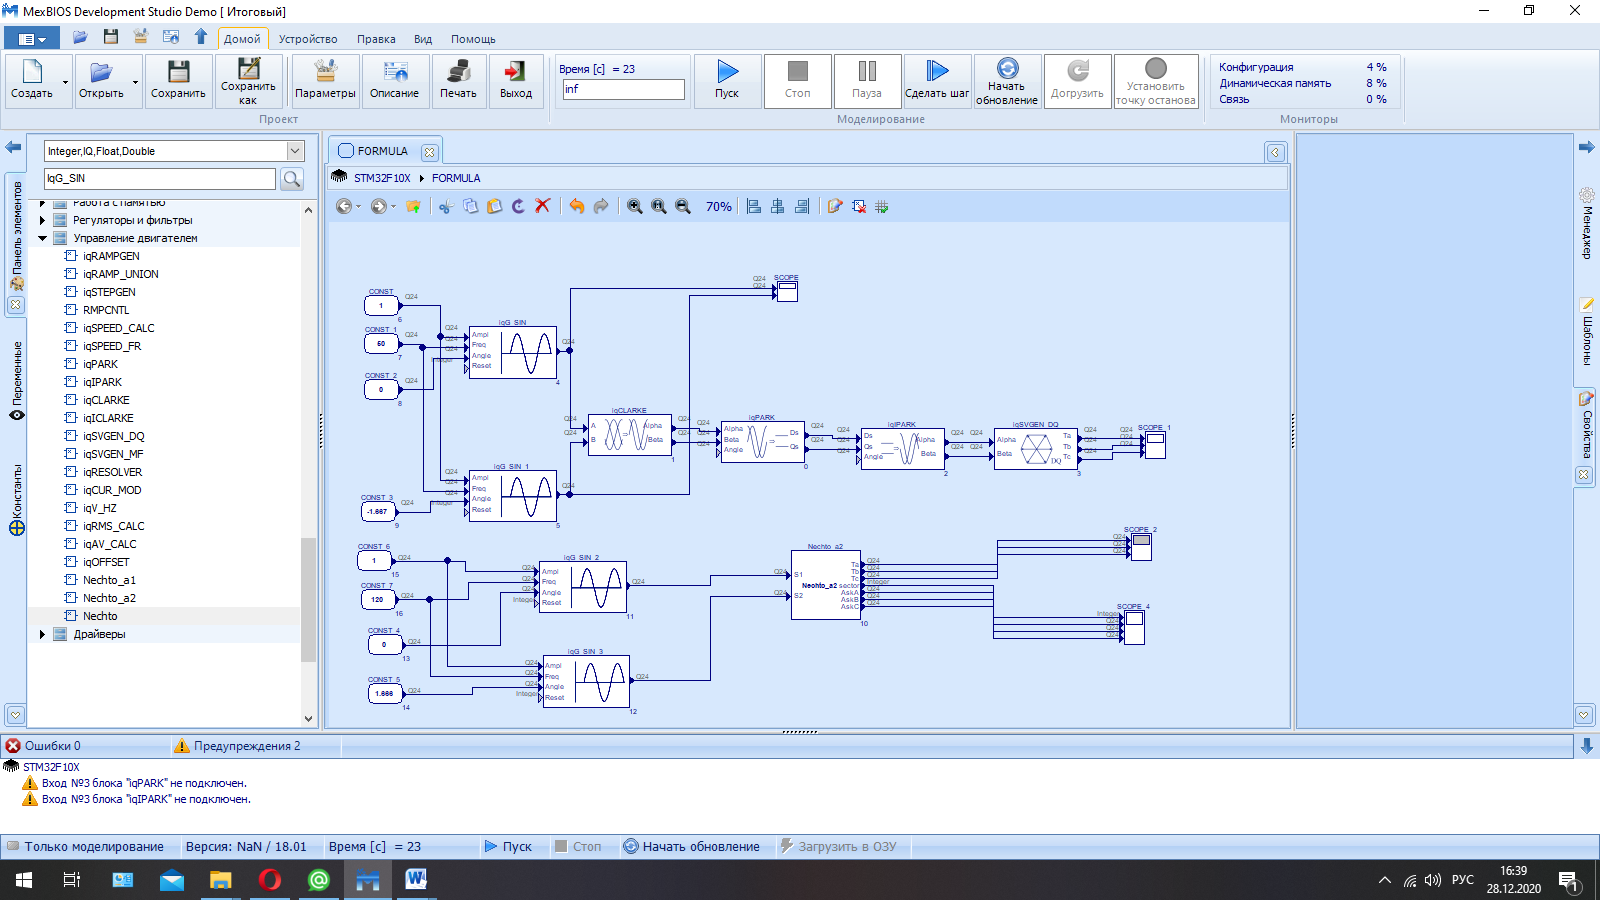
\includegraphics[width=1.3\linewidth]{standart.png} 
\end{frame}

\begin{frame}
\hspace{-1cm}
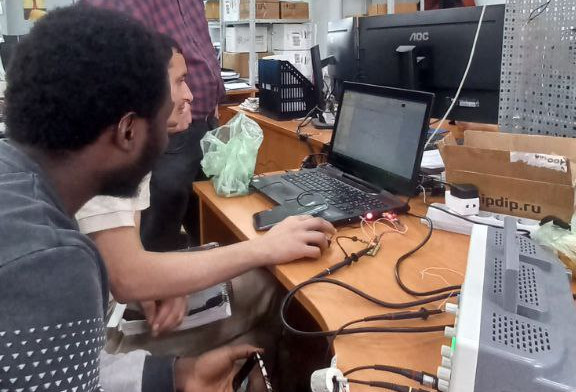
\includegraphics[width=1.1\linewidth]{students.jpg}
\end{frame}

\begin{frame}
\hspace{-1cm}
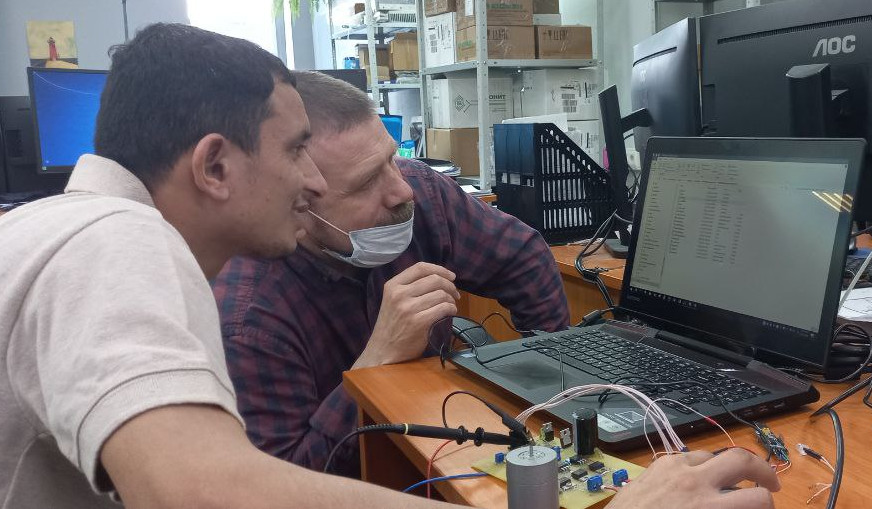
\includegraphics[width=1.1\linewidth]{students1.jpg}
\end{frame}



\begin{frame}
\centering
Спасибо за внимание!
\vspace{1cm}

\url{https://www.overleaf.com/read/gvgvxfhystwk}

\end{frame}



\end{document}


